%%%%%%%%%%%%%%%%%%%%%%%%%%%%%%%%%%%%%%%%%%%%%%%%%%%%%%%%%%%%%%%%%%%%%%%%%%%%%%%%%%%%%%%%%%%%%%%%%%%%%%%%%%%%%%%%%%%%%%%%%%%%%%%%%%%%%%%%%%%%%%%%%%%%%%%%%%%%%%%%%%%
% Written By Michael Brodskiy
% Class: Fundamentals of Electronics
% Professor: I. Salama
%%%%%%%%%%%%%%%%%%%%%%%%%%%%%%%%%%%%%%%%%%%%%%%%%%%%%%%%%%%%%%%%%%%%%%%%%%%%%%%%%%%%%%%%%%%%%%%%%%%%%%%%%%%%%%%%%%%%%%%%%%%%%%%%%%%%%%%%%%%%%%%%%%%%%%%%%%%%%%%%%%%

\include{Includes.tex}

\title{Pre-Lab 3}
\date{October 14, 2024}
\author{Michael Brodskiy\\ \small Professor: M. Onabajo}

\begin{document}

\maketitle

\begin{enumerate}

  \item

    Looking at the provided Figure, and combining with Kirchoff's Voltage Law at the input loop, we may write:

    $$I_b=\frac{V-V_{be}}{R_b}$$

    We know that, when a bit is in the active region, $I_c=\beta I_b$, and $V_{ce}>.2[\si{\volt}]$. We are given that $V_{ce}=3.72[\si{\volt}]$, $V_{be}=.7[\si{\volt}]$, and, based on the figure, $V_{cc}=10[\si{\volt}]$, $R_B=309[\si{\kilo\ohm}]$, and $R_C=1[\si{\kilo\ohm}]$. Thus, we may write:

    $$I_b=\frac{10-.7}{309\cdot10^3}$$
    $$\boxed{I_b=30.097[\si{\micro\amp}]}$$

    Equivalently, for $I_c$:

    $$I_c=\frac{10-3.72}{1000}$$
    $$\boxed{I_c=6.28[\si{\milli\amp}]}$$

    We now find $\beta$:

    $$\beta=\frac{I_c}{I_b}$$
    $$\beta=\frac{6.28}{.030097}$$
    $$\boxed{\beta=208.667}$$

  \item

    We know that the maximum value of $R_B$ may be found for $V_c=V_b$, when the BJT enters saturation mode. For this, we can say $V_c=3.72[\si{\volt}]$, since the emitter is grounded ($V_e=0$), and $V_{ce}$ is given as $3.72[\si{\volt}]$. Thus, we apply KVL to get:

    $$V-I_bR_B=V_B$$
    $$R_B=\frac{V-V_B}{I_b}$$

    We can use the current values found in part (a) to get:

    $$R_B=\frac{10-3.72}{30.097\cdot10^{-6}}$$
    $$R_B=2.0866\cdot10^{5}$$
    $$\boxed{R_B=208.66[\si{\kilo\ohm}]}$$

    The BJT remains in saturation for $R_B\leq 208.66[\si{\kilo\ohm}]$

  \item

    Let us refer to the added resistor as $R_n$. The addition of this resistor forms a voltage divider such that:

    $$V_b=\frac{10R_n}{R_n+R_b}$$

    Since we know $V_b<.3[\si{\volt}]$, we can solve for the cut-off value as:

    $$\frac{10R_n}{R_n+R_b}=.3$$
    $$9.7R_n=.3R_b$$
    $$R_n=.030928R_b$$
    $$\boxed{R_n=9.5567[\si{\kilo\ohm}]}$$

  \item

    We know that, when the light entering the photoresistor is limited, the resistance is very high. Because of this, we need to stop current from entering the base terminal, which would increase its magnitude, but make it more negative. We can do this by connecting the photoresistor to the PNP base. This will result in positive flow from the emitter, which connects to the LED and turns it on. Thus, we can build the following circuit:

    \begin{figure}[H]
      \centering
      \tikzset{every picture/.style={line width=0.75pt}} %set default line width to 0.75pt        

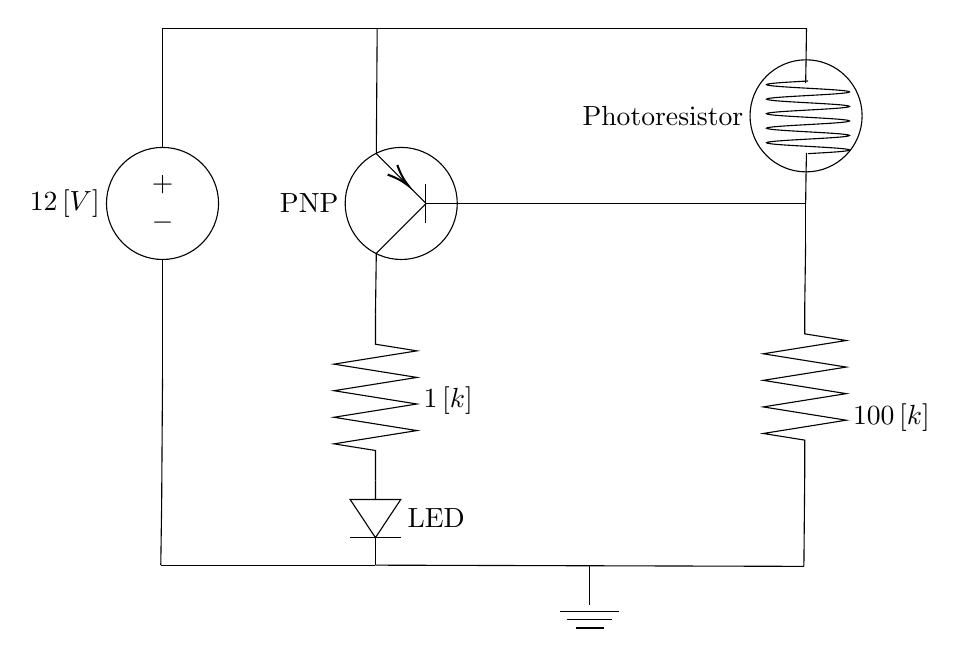
\begin{tikzpicture}[x=0.75pt,y=0.75pt,yscale=-1,xscale=1]
%uncomment if require: \path (0,530); %set diagram left start at 0, and has height of 530

%Shape: Circle [id:dp4569927472871448] 
\draw   (130,208) .. controls (130,193.09) and (142.09,181) .. (157,181) .. controls (171.91,181) and (184,193.09) .. (184,208) .. controls (184,222.91) and (171.91,235) .. (157,235) .. controls (142.09,235) and (130,222.91) .. (130,208) -- cycle ;
%Straight Lines [id:da37823560559477176] 
\draw    (157,123.58) -- (157,181) ;
%Straight Lines [id:da09955128296451543] 
\draw    (157,235) -- (157,292.42) ;
%Shape: Ellipse [id:dp6294239791322914] 
\draw   (299,208) .. controls (299,193.09) and (286.91,181) .. (272,181) .. controls (257.09,181) and (245,193.09) .. (245,208) .. controls (245,222.91) and (257.09,235) .. (272,235) .. controls (286.91,235) and (299,222.91) .. (299,208) -- cycle ;
%Straight Lines [id:da033522493316593405] 
\draw    (284,208) -- (299,208) ;
%Straight Lines [id:da31037866530434155] 
\draw    (283.5,217.5) -- (283.5,198.5) ;
%Straight Lines [id:da3348114195507468] 
\draw    (284,208) -- (275.51,199.51) ;
%Straight Lines [id:da8541070291631819] 
\draw    (260,184) -- (274.1,198.1) ;
\draw [shift={(275.51,199.51)}, rotate = 225] [color={rgb, 255:red, 0; green, 0; blue, 0 }  ][line width=0.75]    (10.93,-3.29) .. controls (6.95,-1.4) and (3.31,-0.3) .. (0,0) .. controls (3.31,0.3) and (6.95,1.4) .. (10.93,3.29)   ;
%Straight Lines [id:da7780110130058856] 
\draw    (284,208) -- (275.51,216.49) ;
%Straight Lines [id:da8564485226781426] 
\draw    (260,232) -- (275.51,216.49) ;
%Straight Lines [id:da22574352758349936] 
\draw    (260.42,123.58) -- (157,123.58) ;
%Straight Lines [id:da8605470966896673] 
\draw    (260.42,123.58) -- (260,184) ;
%Straight Lines [id:da9484987794463876] 
\draw    (259.59,382.27) -- (156.16,382.27) ;
%Straight Lines [id:da8392453680305331] 
\draw    (157,292.42) -- (156.58,352.85) ;
%Shape: Resistor [id:dp21281183062413322] 
\draw   (259.59,261.42) -- (259.59,275.82) -- (279.59,279.02) -- (239.59,285.42) -- (279.59,291.82) -- (239.59,298.22) -- (279.59,304.62) -- (239.59,311.02) -- (279.59,317.42) -- (239.59,323.82) -- (259.59,327.02) -- (259.59,341.42) ;
%Straight Lines [id:da4081841627966426] 
\draw    (260,232) -- (259.59,261.42) ;
%Straight Lines [id:da01359630291295677] 
\draw    (156.58,352.85) -- (156.16,382.27) ;
%Shape: Ground [id:dp9713818138191631] 
\draw   (247.38,350.61) -- (259.59,369) -- (271.79,350.61) -- (247.38,350.61) -- cycle (259.59,341.42) -- (259.59,350.61) ;
%Straight Lines [id:da058325033560085005] 
\draw    (247.38,369) -- (271.79,369) ;
%Straight Lines [id:da365216790376107] 
\draw    (259.59,369) -- (259.59,382.27) ;
%Straight Lines [id:da6958598979675725] 
\draw    (466.85,208) -- (299,208) ;
%Shape: Ellipse [id:dp23662015195546449] 
\draw   (494.06,165.79) .. controls (494.06,150.88) and (481.97,138.79) .. (467.06,138.79) .. controls (452.14,138.79) and (440.06,150.88) .. (440.06,165.79) .. controls (440.06,180.7) and (452.14,192.79) .. (467.06,192.79) .. controls (481.97,192.79) and (494.06,180.7) .. (494.06,165.79) -- cycle ;
%Straight Lines [id:da05382556282727058] 
\draw    (363.84,123.58) -- (260.42,123.58) ;
%Straight Lines [id:da13911979981676093] 
\draw    (467.26,123.58) -- (363.84,123.58) ;
%Straight Lines [id:da7710172062839277] 
\draw    (467.26,123.58) -- (467.06,138.79) ;
%Straight Lines [id:da9215274776799535] 
\draw    (467.26,183.58) -- (467.06,192.79) ;
%Shape: Wave [id:dp652248858608695] 
\draw   (468,149) .. controls (457.75,149.57) and (448,150.12) .. (448,150.75) .. controls (448,151.38) and (457.75,151.93) .. (468,152.5) .. controls (478.25,153.07) and (488,153.62) .. (488,154.25) .. controls (488,154.88) and (478.25,155.43) .. (468,156) .. controls (457.75,156.57) and (448,157.12) .. (448,157.75) .. controls (448,158.38) and (457.75,158.93) .. (468,159.5) .. controls (478.25,160.07) and (488,160.62) .. (488,161.25) .. controls (488,161.88) and (478.25,162.43) .. (468,163) .. controls (457.75,163.57) and (448,164.12) .. (448,164.75) .. controls (448,165.38) and (457.75,165.93) .. (468,166.5) .. controls (478.25,167.07) and (488,167.62) .. (488,168.25) .. controls (488,168.88) and (478.25,169.43) .. (468,170) .. controls (457.75,170.57) and (448,171.12) .. (448,171.75) .. controls (448,172.38) and (457.75,172.93) .. (468,173.5) .. controls (478.25,174.07) and (488,174.62) .. (488,175.25) .. controls (488,175.88) and (478.25,176.43) .. (468,177) .. controls (457.75,177.57) and (448,178.12) .. (448,178.75) .. controls (448,179.38) and (457.75,179.93) .. (468,180.5) .. controls (478.25,181.07) and (488,181.62) .. (488,182.25) .. controls (488,182.88) and (478.25,183.43) .. (468,184) ;
%Straight Lines [id:da6788340354798994] 
\draw    (467.06,192.79) -- (466.85,208) ;
%Straight Lines [id:da3130555580198876] 
\draw    (467.06,138.79) -- (466.85,150) ;
%Straight Lines [id:da3257857772323114] 
\draw    (466.85,227) -- (466.43,256.43) ;
%Straight Lines [id:da7692880472392757] 
\draw    (466.85,227) -- (466.85,208) ;
%Shape: Resistor [id:dp07776598711468374] 
\draw   (466.43,256.43) -- (466.43,270.83) -- (486.43,274.03) -- (446.43,280.43) -- (486.43,286.83) -- (446.43,293.23) -- (486.43,299.63) -- (446.43,306.03) -- (486.43,312.43) -- (446.43,318.83) -- (466.43,322.03) -- (466.43,336.43) ;
%Straight Lines [id:da1344556088215254] 
\draw    (466.43,336.43) -- (466.01,382.85) ;
%Straight Lines [id:da08160552331597515] 
\draw    (466.01,382.85) -- (259.59,382.27) ;
%Straight Lines [id:da351044339856595] 
\draw    (362.8,401.56) -- (362.8,382.56) ;
%Straight Lines [id:da13884984600813988] 
\draw    (377.01,404.56) -- (348.59,404.56) ;
%Straight Lines [id:da8859677625891602] 
\draw    (373.51,408.56) -- (352.09,408.56) ;
%Straight Lines [id:da6907057559316673] 
\draw    (369.51,412.56) -- (356.09,412.56) ;

% Text Node
\draw (157,204.6) node [anchor=south] [inner sep=0.75pt]    {$+$};
% Text Node
\draw (157,211.4) node [anchor=north] [inner sep=0.75pt]    {$-$};
% Text Node
\draw (128,208) node [anchor=east] [inner sep=0.75pt]    {$12\left[\text{V}\right]$};
% Text Node
\draw (243,208) node [anchor=east] [inner sep=0.75pt]   [align=left] {PNP};
% Text Node
\draw (281.59,295.22) node [anchor=north west][inner sep=0.75pt]    {$1\left[\text{k} \si{\ohm}\right]$};
% Text Node
\draw (438.06,165.79) node [anchor=east] [inner sep=0.75pt]   [align=left] {Photoresistor};
% Text Node
\draw (273.79,353.61) node [anchor=north west][inner sep=0.75pt]   [align=left] {LED};
% Text Node
\draw (488.43,303.03) node [anchor=north west][inner sep=0.75pt]    {$100\left[\text{k} \si{\ohm}\right]$};


\end{tikzpicture}

      \caption{Light-Triggered Circuit Implementing PNP, Photoresistor, and LED}
      \label{fig:1}
    \end{figure}

    Note that, with sufficient light to the photoresistor, the resistance decreases, which turns the transistor off, causing the LED to turn off when light is available. Furthermore, note the implementation of a low-value resistor prior to the LED to prevent overloading the diode, and a high resistance value which receives current the diode is in reverse bias. The resistor values given in the diagram are based off of the provided values for photoresistor resistance extrema.

    All we have to do to achieve this is integrate a capacitor, which will need to charge before the LED turns on, or fully discharge after the LED turns off. Thus, we may construct:

    \begin{figure}[H]
      \centering
      \include{Figures/PL3d2}
      \caption{Light-Triggered Circuit Implementing PNP, Photoresistor, and LED with Time-Delay}
      \label{fig:2}
    \end{figure}

    We loosely calculate the 1-second delay be finding the time constant as:

    $$\tau=RC$$

    with the resistor value above the LED:

    $$\tau=1000C$$
    $$C=\frac{1}{1000}$$
    $$C=1[\si{\milli\farad}]$$

  \item Done \textcolor{green}{\checkmark}

\end{enumerate}

\end{document}

